\documentclass[a4paper,12pt]{article}
\usepackage[bahasa]{babel}
\usepackage{graphicx}
\usepackage{multirow}
\usepackage{enumitem}
\usepackage{listings}
\usepackage{adjustbox}
\graphicspath{ {./img/} }
\begin{document}
\title{Laporan Praktikum Statistika Pertemuan 10}
%\author{Aldzikri Dwijayanto Prathama \\ {\small 195410189}}
\author{Aldzikri Dwijayanto Prathama 
	\\195410189}
\makeatletter
\begin{titlepage}
	\begin{center}
		{\huge \bfseries \@title }\\[14ex]
		
\includegraphics[scale=.8]{logo}\\[4ex]
		{\large \@author}\\[20ex]
		{\large \bfseries {SEKOLAH TINGGI MANAJEMEN INFORMATIKA DAN KOMPUTER
				AKAKOM YOGYAKARTA}}
	\end{center}


%{\large \@date} 
\end{titlepage}
\makeatother
%\maketitle
\newpage
\tableofcontents
\newpage
\section{Pembahasan}
Probabilitas adalah kemungkinan yang dapat terjadi dalam suatu peristiwa tertentu. Definisi probabilitas dapat dilihat dari tiga macam pendekatan, yaitu pendekatan klasik, pendekatan frekuensi relatif dan pendekatan subjektif.

\subsection{Praktik}
\subsubsection{Praktik 1}
Pada praktik 1 digunakan pendekatan klasik, menurut pendekatan klasik pada suatu peristiwa random dapat terjadi dalam n cara yang masing-masing memiliki kemungkinan yang sama, dan apabila sejumlah n(B) digunakan untuk cara memberikan hasil B.
\begin{center}
	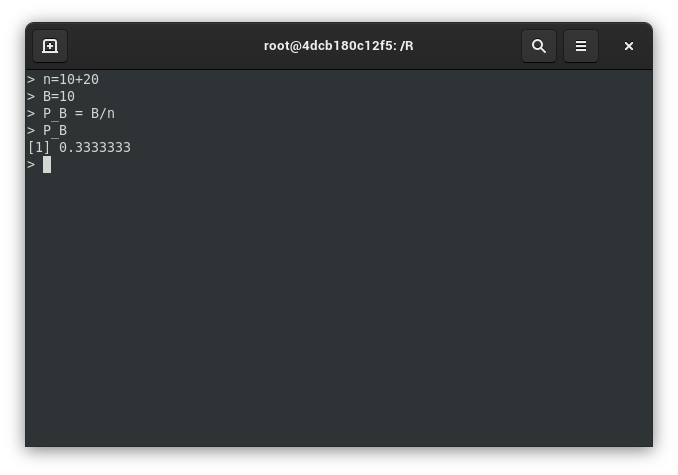
\includegraphics[scale=.5]{prak1}
\end{center}
Pada R Console kita ketikkan\\
\texttt{n=10+20}\\
artinya kita memberi nilai n dengan 10 butir telur bebek ditambah dengan 20 butir telur ayam yaitu 30 butir telur, kemudian klik enter. Selanjutnya kita ketikkan \\
\texttt{B=10}\\
artinya B adalah 10 butir telur. Kemudian kita beri rumus\\ 
\texttt{P\_B = B/n }, kemudian kita panggil lagi P\_B. Maka peluang terambil telur bebek adalah 0,33333.

\subsubsection{Praktik 2}
Praktik 2 adalah menentukan peluang berapa warna merah atau hijau yang terambil dari kotak jika kelereng diambil secara acak dengan mata  tertutup. Diketahui A = mengambil warna merah, B = mengambil warna kuning, C = mengambil warna hijau, n(A) = 10, n(B) = 18, n(C) = 22, dan n = n(A) + n(B) + n(C) = 10+18+22.
\begin{center}
	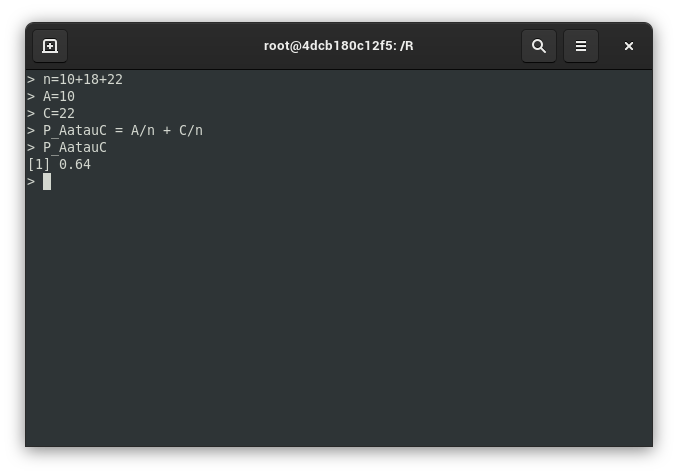
\includegraphics[scale=.5]{prak2}
\end{center} 
Peristiwa tersebut termasuk peristiwa saling lepas. Dua peristiwa atau lebih disebut peristiwa saling lepas apabila kedua atau lebih peristiwa tersebut tidak bisa terjadi pada saat bersamaan. Untuk dua peristiwa A dan peristiwa B yang saling lepas, maka probabilitas terjadinya peristiwa tersebut adalah sebagai berikut:
\[ P(A \cup B) = P(A)+P(B) \]

Jadi pada R Console dibawah kita ketikkan\\ 
\texttt{n=10+18+22}\\
yang artinya kita memberi nilai n dengan 10 kelereng merah ditambah 18 kelereng hijau ditambah 22 kelereng kuning yaitu 50 butir kelereng. Kemudian kita ketikkan\\ 
\texttt{A=10}\\ 
yang artinya A adalah 10 kelereng merah, kemudian kita ketikkan lagi\\ 
\texttt{C=22}\\ 
yang artinya C adalah 22 kelereng kuning, setelah itu kita ketikkan\\  \texttt{P\_AatauC = A/n + C/n}\\ 
Hasil akhir yang didapatkan adalah Peluang terambilnya kelereng warna merah atau kuning adalah 0,64.
 
\subsubsection{Praktik 3}
Praktik 3 adalah menentukan peluang yang terpilih siswa yang menyukai matematika atau bahasa Inggris, dari 45 siswa pada suatu kelas, diketahui 28 siswa senang matematika, 22 siswa bahasa inggris, dan 10 siswa suka kedua-duanya. Jika seorang siswa dipilih secara acak
\begin{center}
	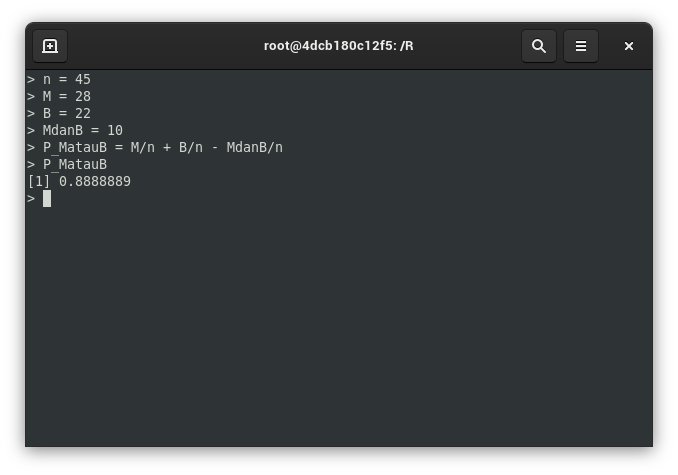
\includegraphics[scale=.5]{prak3}
\end{center}
Peristiwa tersebut termasuk peristiwa tidak saling bebas, karena terjadinya peristiwa yang satu mempengaruhi atau dipengaruhi terjadinya peristiwa yang lainnya. Untuk dua peristiwa A dan B yang tidak saling bebas, probabilitas terjadinya peristiwa tersebut adalah sebagai berikut:
\[ P(A \cap B) = P(A) P(B|A) \]
Diketahui M = suka matematika, B = suka Bahasa inggris, n = 45 artinya banyaknya data dari praktik ini adalah 45, kemudia n(M) = 28 artinya banyaknya yang suka matematika, n(B) = 22 adalah banyaknya yang suka Bahasa inggris, dan n(M Ç B) = 10 artinya banyaknya yang suka keduanya. Dari data tersebut bisa diketahui bahwa Dua atau lebih peristiwa disebut peristiwa tidak saling lepas apabila kedua atau lebih peristiwa tersebut dapat terjadi pada saat yang bersamaan. Maka probabilitas terjadinya peristiwa tersebut adalah 0.88889

\subsubsection{Praktik 4}
Praktik 4 adalah menentukan peluang bahwa jumlah mata kedua dadu lebih dari 3, jika dua buah dadu dilambungkan bersama-sama.
\begin{center}
	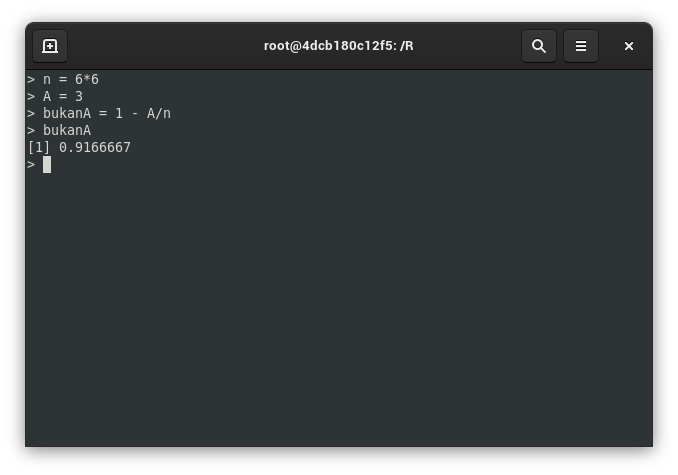
\includegraphics[scale=.5]{prak4}
\end{center}
Dua buah dadu dilambungkan bersama, maka n = 6 x 6 = 36. Jika A = {jumlah mata kedua dadu £ 3} = {(1,1), (1,2), (2,1)}. Kemudian untuk n(A) = 3, dan B = {jumlah mata kedua dadu > 3}. Bisa dilihat pada R Console dibawah, kita ketikkan n=6*6. Kemudian kita ketikkan A=3 yang artinya jumlah mata dadu sama dengan 3. Setelah itu kita ketikkan > bukanA = 1 – A/n, kemudian kita panggil > bukanA , maka peluang bahwa jumlah mata kedua dadu > 3 adalah 0,9167.

\end{document}